\documentclass[tikz,border=4pt]{standalone}
\usepackage[T1]{fontenc}
\usepackage[utf8]{inputenc}
\usepackage{amsmath,amssymb}
\usepackage{helvet}
\renewcommand{\familydefault}{\sfdefault}
\usepackage{pgfplots}
\pgfplotsset{compat=1.17}
\usetikzlibrary{arrows.meta,positioning,calc,fit,backgrounds,shapes.geometric}

\definecolor{cVis}{HTML}{1F77B4}
\definecolor{cTxt}{HTML}{D62728}
\definecolor{cProj}{HTML}{2CA02C}
\definecolor{cLLM}{HTML}{9467BD}
\definecolor{cConv}{HTML}{FF7F0E}
\definecolor{cAtt}{HTML}{17BECF}
\definecolor{cGray}{HTML}{7F7F7F}

\tikzset{
  blk/.style={draw, rounded corners=2pt, minimum height=8mm, align=center, font=\footnotesize, thick},
  tok/.style={draw, minimum size=3.2mm, inner sep=0pt},
  arr/.style={-{Stealth[length=2mm]}, thick},
}

\begin{document}
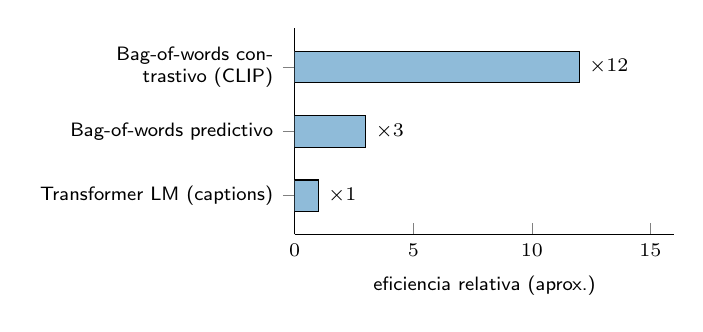
\begin{tikzpicture}
  \begin{axis}[
    xbar, width=6.4cm, height=4.2cm, xmin=0, xmax=16,
    symbolic y coords={lm,bow,clip}, ytick=data, yticklabels={Transformer LM (captions),Bag-of-words predictivo,Bag-of-words contrastivo (CLIP)}, yticklabel style={font=\scriptsize, align=right, text width=3.0cm},
    xlabel={\scriptsize eficiencia relativa (aprox.)}, xticklabel style={font=\scriptsize},
    nodes near coords={\scriptsize$\times$\pgfmathprintnumber\pgfplotspointmeta}, nodes near coords align={horizontal},
    bar width=4mm, enlarge y limits=0.3, axis lines*=left]
    \addplot[fill=cVis!50] coordinates {(1,lm) (3,bow) (12,clip)};
  \end{axis}
\end{tikzpicture}
\end{document}
